\chapter{Antecedentes}

A principios del milenio el grupo GITEM inició un estudio para abordar problemas puntuales en la implementación de servicios médicos prestados a través de medios teleinformáticos en el Distrito Capital\cite{aparicio2000}:

\begin{quote}
“En el momento no existe un diagnóstico real sobre los servicios requeridos en el área de telemedicina, razón suficiente para iniciar un trabajo de campo que establezca la situación actual de servicios médicos y la demanda real, así como la posibilidad de conocer a corto, mediano y largo plazo cuáles serían los costos de inversión que permitirían dar soluciones al problema  de cobertura.

La socialización del conocimiento alrededor de las tecnologías aplicadas al desarrollo de la medicina, es uno de los valores que lleva al éxito de soluciones efectivas en el sector salud, por tal motivo es necesario desarrollar un plan de alfabetización en el sector salud y en el sector gubernamental y académico.

En el país no existen estrategias de investigación en esta área del conocimiento para llevar a cabo un estudio real que permita dar el paso a soluciones verdaderas sobre desarrollo tecnológico o experimental para poder implementar centros de investigación en Telemedicina.

La Universidad Distrital tiene el recurso humano, el conocimiento y la experiencia científica y tecnológica, capaz de dar soluciones tangibles a estas necesidades; unida al conocimiento y experiencia de entidades como clínicas y hospitales  y con la participación de operadores de comunicaciones, puede desarrollar soluciones efectivas a los problemas de salud que afronta la sociedad colombiana.”
\end{quote}

Para facilitar el aprovechamiento del estudio, los resultados obtenidos fueron recopilados en extensos tomos en formato físico y digital. Aunque totalmente eficaz en primera instancia, los resultados obtenidos no tenían una estructura documental coherente ni un modelo de información que los caracterizara. Este hecho, a la par con el ingreso de entidades al estudio, aumentó la complejidad a la hora de generar estudios comparativos o de apoyo a la toma de decisiones, teniéndose en muchos casos información faltante, redundante e innecesaria para el proyecto. Dado que la muestra objeto de estudio es intrínsecamente  dinámica, cualquier cambio de la condiciones iniciales es difícilmente reflejado, quedando en poco tiempo la información desactualizada. En ese escenario, la labor de articular las prestaciones de las organizaciones suponía un proceso lento y la estrategia de gestión de información empleada en el estudio comenzó a mostrar debilidades.

Respondiendo a este nuevo contexto problémico se creó al interior del grupo un proyecto de grado denominado \textbf{Sistema de Información para la Caracterización de Proyectos de eSalud} que en sus primeras fases de desarrollo dio solución parcial al marcar las pautas hacia la integración de información para el \textbf{GITEM}, dejando además una investigación valiosa en el tema del desarrollo de software distribuido, interoperable y robusto basado en la filosofía del software libre. En paralelo el grupo de investigación implementó, en convenio con \textit{Colciencias}, el Sistema de Referencia y Contrarreferencia para el Distrito Capital, utilizando herramientas de desarrollo propietarias específicamente el middleware .NET de Microsoft con lo que el grupo adquirió experiencia en la desarrollo de aplicaciones siguiendo metodologías efectivas para la construcción de software.

\section{Fases Transcurridas en el SITEM}
SITEM es un proyecto de investigación asociado a un holotipo proyectivo\cite{hurtado2000}. El estadio actual se ha logrado a partir de actividades investigativas que abordan distintos aspectos de la proyección y diseño de sistemas de eSalud. La idea fundamental del proyecto es la de generar un proceso iterativo basado en la construcción y deconstrucción gradual, hermenéutico e incremental de un sistema que apoye las labores de consultoría y diseño de redes de telesalud, ahondando de forma asíncrona cada uno de sus componentes. 

El proyecto tiene como particularidad que tiene que cumplir con los requisitos planteados empleando reducidos recursos técnicos y financieros, los cuales deben ser administrados dentro de un ambiente de alta regulación burocrática. El escenario común ha sido el bajo tiempo de permanencia de los integrantes, la ejecución constante de tareas de capacitación, el uso intensivo de tecnologías de la comunicación, el teletrabajo  y la escasa interacción persona a persona. El \textbf{SITEM} inicialmente tenía que ser de calidad, económico y desarrollado rápidamente. Sien embargo, tal como lacónicamente \cite{larman2003} expresaba: “Rápido, barato, bueno: elija dos cualquiera”; con los pies firmemente puestos en el suelo,  dejando a un lado las fuertes esperanzas, debíamos sacrificar un aspecto y el único que se disponía era la rapidez en que versiones estables del proyecto habrían de ver la luz. Se presupone que  los conceptos fundamentales de desarrollo de aplicaciones de software libre aportaran varias claves para minimizar el impacto de este sacrificio.

\begin{figure}
 \centering
 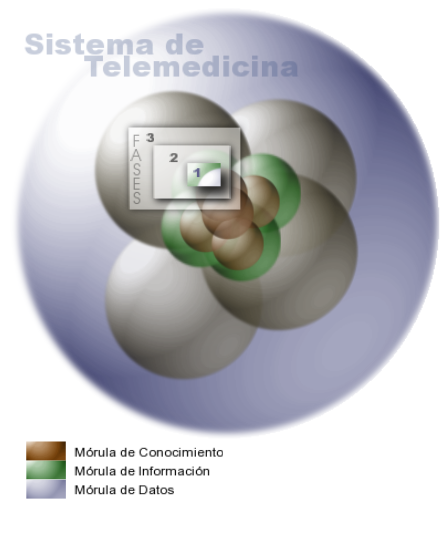
\includegraphics[width=156mm, height=195mm]{modelo_fases.png}
 \caption{Aproximación incremental a un sistema de Gestión de Conocimiento}
 \label{modelo1}
\end{figure}

El grupo plantea un modelo general en donde los objetivos de producir datos, consumir información y compartir conocimiento en el área de interés, será alcanzado en varias fases\footnote{A través del presente documento se utilizan los términos de fase en el proceso investigativo y fases del Proceso de Desarrollo del Sistema Software. Las dos se suponen diferentes y su interpretación e importancia están asociados al contexto en el que se ubican.} de las cuales este documento describe aquellas que han culminado.

La figura \ref{modelo1} muestra el proceso de estructuración del sistema como una sucesión de fases que generan dimensiones de datos, información y conocimiento de un componente. El sistema visto como un \textit{holos} presenta al investigador una gran cantidad de datos que en la medida que se descubren, recolectan, observan y registran se van convirtiendo en información susceptible de ser descrita, analizada, integrada y comparada acercándose cada vez más a un conocimiento refinado. El carácter de discernible - el momento en que las dimensiones se solapan en grado sumo, se evidencia con el aumento colectivo de especialización en la materia y en nuestro caso, con el grado de inmersión que los usuarios del SITEM tengan a partir de la liberación de la versión 1.0 estable (octubre de 2017).

En el transcurso de las fases solo se manejan ciertos aspectos que incrementalmente crean un modelo más refinado del sistema, con base en las diferentes \textit{mórulas} de datos, información y conocimiento generadas. Aunque en el gráfico se muestra un tanto discretos y exactos, los límites existentes entre las tres mórulas principales - datos, información, conocimiento; son en la realidad difusos. Si se consideran los aspectos meramente técnicos del SITEM se corre el riesgo inminente de diseminación en regiones poco profundas del sistema - dispersión en la mórula de datos - razón por la cual la herramienta software se ha convertido en un artefacto intermedio y no en el fin último de la investigación.

\subsection{Sistema de Información para la Caracterización de Proyectos de eSalud – Fase I}
Con la primera fase  se logró un conocimiento amplio de los componentes de las redes de telesalud y sus interrelaciones basado en una investigación exploratoria y descriptiva realizada por los integrantes del grupo. También se determinaron las características esenciales de diferentes portales que implementaban en cierto grado la funcionalidad esperada para el SITEM vislumbrando con este estudio la necesidad de integrar un producto software adaptado a las necesidades del entorno distrital, teniendo en cuenta que ninguno de los portales analizados, permitía la gestión y análisis de información pertinente, confiable, actualizada y estructurada en torno a las redes de telesalud en idioma español.

Esta fase definió un modelo para la estructuración y administración de información relevante para los interesados en el diseño, análisis y desarrollo de redes de eSalud. Además se definió un modelo de negocios que lograba mostrar las interrelaciones que tendría el sistema con los proyectos del grupo y un conjunto representativo de portales relacionados temáticamente; encontrando \textit{un costo de oportunidad adecuado ya que en la actualidad ningún portal se especializa en el proceso de diagnóstico de capacidad para la implementación de eSalud.} No obstante, al momento de desarrolló de esta fase el grupo de investigación no contaba ni siquiera con un portal web por lo que la arquitectura propuesta incluyó al portal del grupo como un subsistema del SITEM, compartiendo de esta forma tanto la plataforma tecnológica como el modelo conceptual, lo que difuminó un poco los alcances reales del Sistema y su implementación no pasó de ser un prototipo de baja funcionalidad. 

Los alcances y logros efectivos de esta fase fueron:

\begin{itemize}
\item Descripción del Modelo de Negocio.
\item Propuesta de Desarrollo
\item Creación de la Arquitectura general del Sistema.
\item Desarrollo del sitio web del grupo GITEM e integración conceptual del SITEM dentro de los proyectos del grupo.
\item Elaboración de los Modelos básicos de Requisitos, análisis y diseño.
\item Estudios sobre filosofía de Software Libre.
\item Construcción de un Prototipo de baja funcionalidad conocido como SITEM versión 0.1, bautizada internamente como \textbf{Kauil}.
\end{itemize}


\begin{figure}
 \centering
 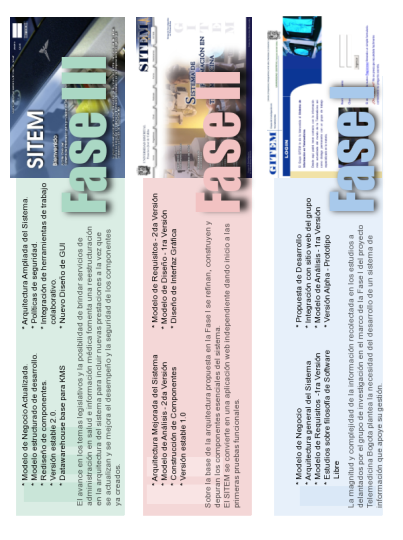
\includegraphics[width=142mm, height=190mm]{fase_sitem.png}
 \caption{Fases transcurridas en el desarrollo del SITEM}
 \label{fase_sitem}
\end{figure}

\subsection{Sistema de Información para la Caracterización de Proyectos de eSalud – Fase II}

Los modelos de requisitos, análisis y diseño de la primera fase sirvieron de base para proponer arquitectura general para el Sistema de Información para la Caracterización de Proyectos de eSalud y con el inicio de la segunda fase se emprenden las actividades necesarias para la integración de los componentes de software que concretaban dicha arquitectura. Para poder minimizar los riesgos asociados al proyecto se adaptó el \textit{OpenUP} a las especificidades de desarrollo del Sistema, lo que favoreció efectivamente su elaboración, implementación, mantenimiento y crecimiento.

La arquitectura general se vio poco afectada, pero cada uno de los subsistemas componentes fueron finamente caracterizados. Esto generó un modelo de análisis y diseño definido que integraba elementos no tratados en la fase inicial. Debido a la naturaleza del SITEM, el grupo de investigación decide separar los hilos de desarrollo del Sistema y del proceso de estructuración del sitio web del grupo. El SITEM por primera vez se puede acceder desde \textit{Internet} gracias al despliegue que se realiza sobre la plataforma de hardware y software brindada por la \textit{Universidad Distrital}. 

En esta fase se realiza el modelado de datos y se esbozan las primeras rutinas de manejo se seguridad. Para la integración de componentes se utilizan herramientas de software libre y el grupo de desarrollo aumenta a cinco integrantes. El trabajo se encuentra, con excepción del director del proyecto, soportado y ejecutado por estudiantes de pregrado del proyecto curricular de Ingeniería Electrónica convirtiéndose en el \textbf{primer proyecto de desarrollo de software libre realizado por el GITEM}.

Los alcances de esta fase fueron:
\begin{itemize}
\item Arquitectura Mejorada del Sistema
\item Modelo depurado de Requisitos
\item Modelo de Análisis - Segunda Versión
\item Modelo de Diseño
\item Construcción de Componentes software soportado en su totalidad por herramientas de software libre.
\item Diseño de Interfaz Gráfica
\item Versión 0.5 beta bautizada internamente como \textbf{Gucumatz}.
\item Adaptación del OpenUP a las especificidades del SITEM.
\item Configuración de la plataforma tecnológica de despliegue del sistema.
\end{itemize}

Al final de la fase se obtiene un aplicativo que presenta avances en todos los subsistemas propuestos.


\subsection{Sistema de Información para la Caracterización de Proyectos de eSalud – Fase III}

En esta fase se especializa la categoría del SITEM como un sistema de inteligencia empresarial analítica. La arquitectura del sistema se enriquece con componentes relacionados con inteligencia de negocio tales como gestión de indicadores claves de desempeño, seguimiento automatizado de desempeño, cuadros de mando integrales, tableros de comando, Procesamiento Analítico en Línea (OLAP), minería de datos, búsqueda por ejemplo, entre muchos otros.

En esta fase el grupo toma una decisión arquitectónica importante y concentra su esfuerzo en el motor de integración de aplicaciones, cuyo objetivo es la federación de sistemas existentes de software libre o código abierto (FLOSS) con el objetivo de lograr un mayor nivel funcional del que se había alcanzado en las fases anteriores. Se trata de buscar el aseguramiento de la calidad en el desarrollo, la interoperabilidad, escalabilidad y el uso extensivo de FLOSS. Se documenta todas las etapas involucradas en la creación de la aplicación para que sirva de plantilla a sistemas relacionados y se formaliza las áreas de capacitación a partir de ciclos genéricos de transferencia de conocimiento apoyados en tecnologías de la información.

Es precisamente esta fase la que da vida a este documento, a una arquitectura emergente y una versión 1.0 del sistema denominada OpenSITEM, con la que el grupo entrega un sistema complejo constituido por un motor de federación - basado en SARA un framework de desarrollo para plicaciones web desarrollado por el grupo; que articula las herramientas externas Knowage, ERPNext, Alfresco Community, CAMUNDA y OpenProject, así como varias herramientas propias tales como el Sistema Integrado de Autoevaluación. OpenSITEM presenta al usuario final una interfaz unificada que soporta los flujos de trabajo definidos. 

\begin{figure}
 \centering
 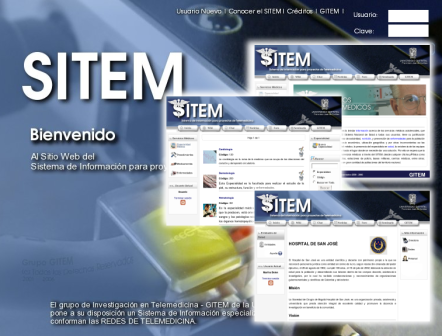
\includegraphics[width=156mm, height=118mm]{pagina_principal.png}
 \caption{Sistema de Información para la Caracterización de Proyectos de eSalud. Interfaz de Usuario en la Fase III}
 \label{sitem_faseIII}
\end{figure}